\subsection{Vorwärtspropagation in Neuronalen Netzwerken}
\label{sec: Forward Propagation}
Die Vorwärtspropagation ist ein wesentlicher Prozess in neuronalen Netzwerken, der die Übertragung von Eingabedaten durch die Netzwerkarchitektur ermöglicht, um die Ausgabe zu erzeugen \cite{russell2021ai}. 
Sie ist eine Abfolge von mathematischen Operationen, die Gewichtungen, Biases und Aktivierungsfunktionen beinhalten \cite{Chollet2021}.
Dieser Abschnitt zielt darauf ab, die Schlüsselelemente und mathematischen Grundlagen zu diskutieren, die die Vorwärtspropagation beeinflussen und stellt aktuelle Forschungsergebnisse und praktische Implikationen vor.
%
\subsubsection{Schicht-für-Schicht-Propagation}

Die Vorwärtspropagation beginnt bei den Eingabedaten \( X \), bezeichnet als \( A^{[0]} \). In jeder Schicht wird aus dem Ausgang \( A^{[l-1]} \) der vorherigen Schicht ein Vektor \( Z^{[l]} \) berechnet. Die Werte für jede nachfolgende Schicht \( A^{[l]} \) werden entsprechend der Gleichung (\ref{eq:forward}) ermittelt. Dieser Prozess wiederholt sich von Schicht zu Schicht und bildet das Kernstück der Vorwärtspropagation.
%
\begin{equation}
Z^{[l]} = W^{[l]} A^{[l-1]} + b^{[l]}
\label{eq:forward}
\end{equation}
%
%
%
%
\subsubsection{Aktivierungsfunktionen}
Aktivierungsfunktionen in neuronalen Netzen spielen eine entscheidende Rolle, indem sie die gewichtete Summe \( Z^{[l]} \) in einen aktivierten Ausgabewert \( A^{[l]} \) umwandeln. Diese Transformation wird typischerweise durch \( \sigma \) dargestellt, wie in der folgenden Gleichung gezeigt:
%
\begin{equation} \label{eq:activation_function}
A^{[l]} = \sigma(Z^{[l]})
\end{equation}
%
\begin{figure}[htbp]
  \centering
  \begin{subfigure}{0.45\textwidth}
    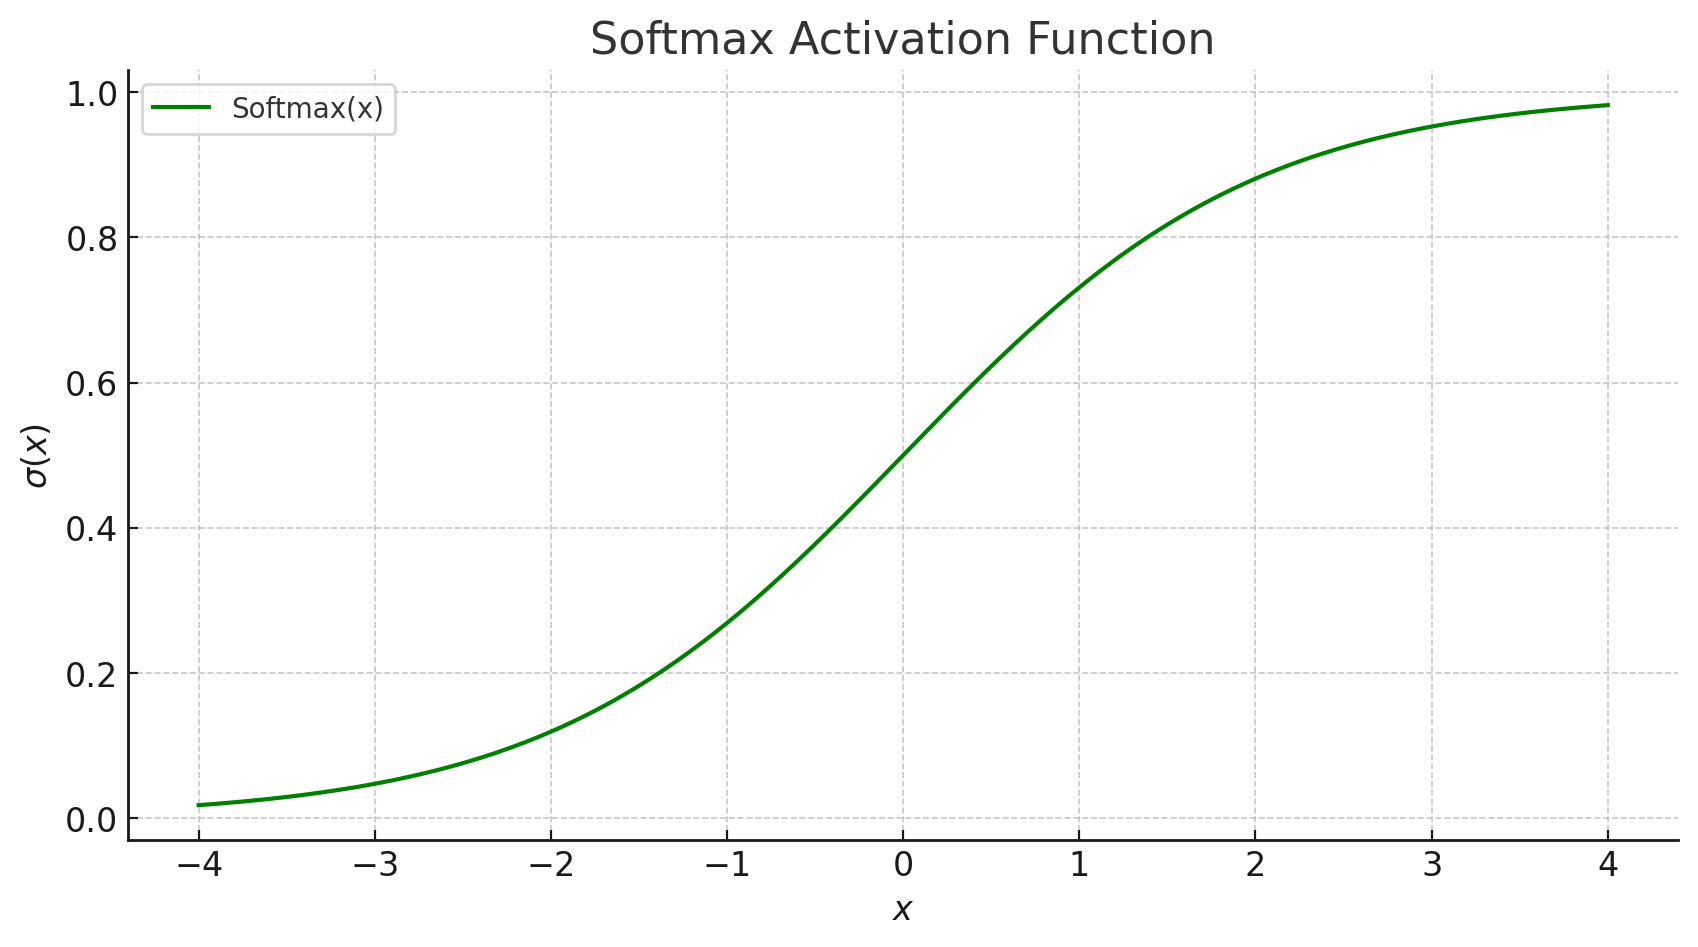
\includegraphics[width=\textwidth]{2Grundlagen/22SoftMax.png}
    \caption{Softmax-Funktion}
    \label{fig:softmax}
  \end{subfigure}
  \hfill
  \begin{subfigure}{0.45\textwidth}
    \includegraphics[width=\textwidth]{2Grundlagen/22ReLU.png}
    \caption{ReLU-Funktion}
    \label{fig:relu}
  \end{subfigure}
  \caption{Vergleich der Softmax- und ReLU-Aktivierungsfunktionen.}
\end{figure}
%
\paragraph{ReLU-Aktivierungsfunktion}
Die ReLU (Rectified Linear Unit) Aktivierungsfunktion, dargestellt in Abbildung \ref{fig:relu}, ist eine der am häufigsten verwendeten Aktivierungsfunktionen in neuronalen Netzen. Sie wird definiert als \( f(x) = \max(0, x) \) und ist besonders effektiv, um Nichtlinearitäten in den Daten zu modellieren.
%
\begin{equation} \label{eq:relu}
f(x) = \max(0, x)
\end{equation}
%

\paragraph{Softmax-Aktivierungsfunktion}
Die Softmax-Funktion ist eine Aktivierungsfunktion, die häufig in der Ausgabeschicht von Klassifizierungsnetzwerken verwendet wird. Sie wandelt einen Vektor von reellen Zahlen in Wahrscheinlichkeiten um. Die Formel für die Softmax-Funktion ist:
%
\begin{equation} \label{eq:softmax}
\text{Softmax}(z) = \frac{e^{z}}{\sum e^{z}}
\end{equation}
%
Hierbei steht \( e^{z} \) für den Exponentialwert jedes Elements im Vektor \( z \), und der Nenner ist die Summe aller Exponentialwerte im Vektor. Diese Umwandlung stellt sicher, dass die Ausgaben des Netzwerks als Wahrscheinlichkeiten interpretiert werden können, wobei die Summe aller Wahrscheinlichkeiten 1 ergibt.
%
%
\subsubsection{Gewichtsmatrix \( W^{[l]} \) und Bias-Vektor \( b^{[l]} \)}
Die Gewichtsmatrix für die Schicht \( l \) wird als \( W^{[l]} \) bezeichnet, und \( b^{[l]} \) ist der Bias-Vektor für dieselbe Schicht \cite{heaton_2012}. 
Diese Parameter werden während des Backpropagation-Prozesses trainiert, um den Fehler zwischen der vorhergesagten und der tatsächlichen Ausgabe zu minimieren \cite{aggarwal_neural_networks_2018}.
%
\begin{equation}
A^{[l]} = \sigma \left( 
\begin{pmatrix}
w_{1,1}^{[l-1,l]} & w_{1,2}^{[l-1,l]} & \cdots & w_{1,m}^{[l-1,l]} \\
w_{2,1}^{[l-1,l]} & w_{2,2}^{[l-1,l]} & \cdots & w_{2,m}^{[l-1,l]} \\
\vdots & \vdots & \ddots & \vdots \\
w_{n,1}^{[l-1,l]} & w_{n,2}^{[l-1,l]} & \cdots & w_{n,m}^{[l-1,l]}
\end{pmatrix}
\begin{pmatrix}
A_1^{[l-1]} \\
A_2^{[l-1]} \\
\vdots \\
A_m^{[l-1]}
\end{pmatrix}
+
\begin{pmatrix}
b_1^{[l]} \\
b_2^{[l]} \\
\vdots \\
b_n^{[l]}
\end{pmatrix}
\right)
	\label{eq:forward_big}
\end{equation}
%
\subsubsection{Matrix-Vektor-Operationen und Parallelität}
%
Die Gleichung (\ref{eq:forward_big}) illustriert die Verarbeitungsschritte während der Vorwärtspropagation in neuronalen Netzwerken. 
Eine besondere Stärke dieser Darstellung ist die Visualisierung der Matrix-Vektor-Operationen. 
Diese Operationen sind von Natur aus parallel, was bedeutet, dass sie mehrere Berechnungen gleichzeitig durchführen können. 
Dies zeigt sich besonders in der Matrixmultiplikation, bei der jede Zeile der Gewichtsmatrix gleichzeitig mit dem Aktivierungsvektor multipliziert wird.
%
In modernen Computerarchitekturen, insbesondere bei Grafikprozessoren (GPUs), kann diese inhärente Parallelität der Matrix-Operationen effektiv ausgenutzt werden, um die Berechnungsgeschwindigkeit erheblich zu steigern. 
Das bedeutet, dass die Berechnungen von \( Z^{[l]} \) und \( A^{[l]} \) simultan für alle Neuronen in Schicht \( l \) durchgeführt werden können. Dies ist ein entscheidender Vorteil, insbesondere in tiefen Netzwerken mit vielen Schichten und Neuronen.
%
Die Verwendung der Matrixnotation erleichtert nicht nur das Verständnis der Struktur und des Arbeitsablaufs eines neuronalen Netzwerks, sondern hebt auch die Möglichkeit hervor, leistungsstarke parallele Hardwarearchitekturen effizient zu nutzen.
%
%
